\section{Experiments / Results / Discussion}

\textbf{Random Forest Model:} The results from the Random Forest model, with a training
MSE of 1.92 and test MSE of 2.37, and $R^{2}$ scores of 0.77 for training and
0.72 for testing, indicate moderate predictive performance.

\begin{table}[h!]
	\centering
	\caption{Random Forest Model Performance Metrics}
	\renewcommand{\arraystretch}{1} % Adjust row height for better readability
	\setlength{\tabcolsep}{10pt} % Adjust column spacing
	\begin{tabular}{|c|c|c|}
		\hline
		\textbf{Metric} & \textbf{Training} & \textbf{Test} \\
		\hline
		MSE             & 1.92              & 2.37          \\
		\hline
		$R^{2}$         & 0.77              & 0.72          \\
		\hline
	\end{tabular}
\end{table}

The small gap between the training and test metrics shows that the Random Forest
model avoids overfitting, which is a positive outcome. However, the $R^{2}$ value
of 0.72 for the test set indicates that nearly 28\% of the variance remains
unexplained, suggesting there is room for improvement in predictive accuracy.
Additionally, Random Forest, while robust, treats each tree independently and averages
their results, which can sometimes limit its ability to capture complex
relationships or interactions in high-dimensional data.

The Random Forest model serves as a strong baseline, demonstrating good generalization
and predictive capacity. However, the unexplained variance and potential limitations
in capturing complex feature interactions make XGBoost a compelling next step.
With its advanced boosting mechanism, regularization capabilities, and efficient
handling of high-dimensional data, XGBoost offers the potential to achieve higher
accuracy and better $R^{2}$ scores, ultimately leading to more reliable
predictions for the finished lot price to land value ratio.

\textbf{Final Model Training Details:} The final machine learning regression model
underwent an extensive hyperparameter tuning process, involving 5-fold cross-validation
over 972 hyperparameter combinations, resulting in a total of 4860 fits. This
thorough optimization ensures that the model achieves both robust performance
and generalizability.

\begin{minipage}[t]{0.48\textwidth}
	\centering
	\captionof{table}{Best Hyperparameters for the Model}
	\renewcommand{\arraystretch}{1} % Adjust row height
	\setlength{\tabcolsep}{8pt} % Adjust column spacing
	\begin{tabular}{|l|c|}
		\hline
		\textbf{Parameter Name}                 & \textbf{Value} \\
		\hline
		\texttt{regressor\_\_colsample\_bytree} & 0.4            \\
		\hline
		\texttt{regressor\_\_learning\_rate}    & 0.1            \\
		\hline
		\texttt{regressor\_\_max\_depth}        & 10             \\
		\hline
		\texttt{regressor\_\_n\_estimators}     & 700            \\
		\hline
		\texttt{regressor\_\_reg\_alpha}        & 0.5            \\
		\hline
		\texttt{regressor\_\_reg\_lambda}       & 0              \\
		\hline
		\texttt{regressor\_\_subsample}         & 1.0            \\
		\hline
	\end{tabular}
\end{minipage}%
\hfill
\begin{minipage}[t]{0.48\textwidth}
	\centering
	\captionof{table}{Model Performance Metrics}
	\renewcommand{\arraystretch}{1} % Adjust row height
	\setlength{\tabcolsep}{10pt} % Adjust column spacing
	\begin{tabular}{|c|c|c|}
		\hline
		\textbf{Metric} & \textbf{Training} & \textbf{Test} \\
		\hline
		MSE             & 2.06              & 3.66          \\
		\hline
		$R^{2}$         & 0.91              & 0.85          \\
		\hline
	\end{tabular}
\end{minipage}

The optimized hyperparameters include a maximum depth of 10 for the decision
trees, allowing the model to capture complex patterns without overfitting. The
learning rate was set to 0.1, providing a balanced trade-off between convergence
speed and model stability. Regularization parameters (\texttt{reg\_alpha} and
\texttt{reg\_lambda}) were adjusted to reduce overfitting, with \texttt{reg\_alpha}
set to 0.5 and \texttt{reg\_lambda} set to 0. The model also used a subsample value
of 1.0 and a \texttt{colsample\_bytree} value of 0.4, ensuring sufficient diversity
in the trees while controlling complexity.

The slight drop in performance from the training to the test set suggests the model
generalizes well, but it also indicates there may still be minor overfitting or
limitations in capturing the full variability of unseen data.

\begin{figure}[h!]
	\centering
	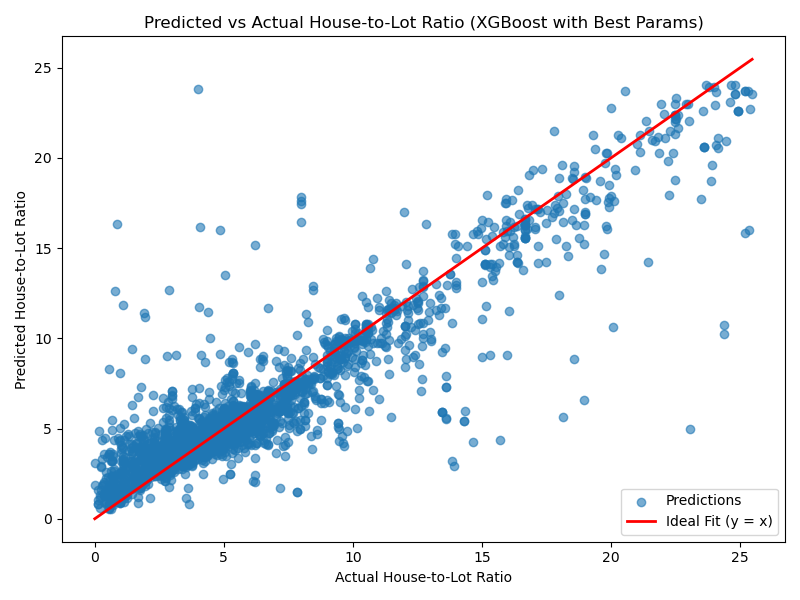
\includegraphics[width=0.3\textwidth]{
		Sections/Final Model.png
	} % Replace with your image path
	\caption{Predicted vs Actual House-to-Lot Ratio}
\end{figure}